% Page 71 start

\chapter{Πίνακες μετασχηματισμών στο χώρο τριών διαστάσεων}

\section{Γεωμετρικοί μετασχηματισμοί}

\subsection{Μεταφορά}

\begin{figure}[hbt]
  \begin{center}
	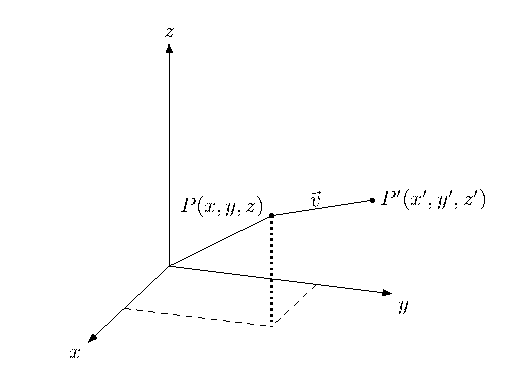
\includegraphics[scale=1]{Chapter3/point-transformation.pdf}
  \end{center}
  \caption{Μεταφορά σημείου σε τρισδιάστατες συντεταγμένες}
\end{figure}



Έστω \( v = (t_x, t_y, t_z) \) τότε \( P' = T_v(P) \) με \( x' = x + t_x \), \( y' = y + t_y \), \( z' = z + t_z \). Το σημείο \((x, y, z)\) σε ομογενείς συντεταγμένες γράφεται:

\[
\begin{bmatrix}
x \\
y \\
z \\
1
\end{bmatrix}
\]

Ο πίνακας μετασχηματισμού της μεταφοράς θα είναι:

\[
T_v =
\begin{bmatrix}
1 & 0 & 0 & t_x \\
0 & 1 & 0 & t_y \\
0 & 0 & 1 & t_z \\
0 & 0 & 0 & 1
\end{bmatrix}
\]

\subsubsection{Μετασχηματισμός κλίμακας}

\( P' = S_{S_x, S_y, S_z} (P) \) με \( x' = S_x \cdot x \), \( y' = S_y\cdot y \) και \( z' = S_z \cdot z \)

Ο πίνακας μετασχηματισμού είναι:

% Page 72 start

\[
S_{S_x, S_y, S_z} = 
\begin{bmatrix}
S_x & 0 & 0 & 0 \\
0 & S_y & 0 & 0 \\
0 & 0 & S_z & 0 \\
0 & 0 & 0 & 1
\end{bmatrix}
\]


\section{Στροφή}

Στον χώρο τριών διαστάσεων για τη στροφή ενός αντικειμένου απαιτούνται δύο παράμετροι:

\begin{enumerate}
    \item[α)] \underline{η γωνία στροφής $\theta$} και
    \item[β)] \underline{ο άξονας περιστροφής του αντικειμένου.}
\end{enumerate}

Οι "κανονικές" στροφές ορίζονται στον χώρο σαν στροφές γύρω από τους θετικούς άξονες $x$, $y$ και $z$.

Για την περίπτωση του θετικού άξονα $z$ έχουμε εάν το σημείο είναι στο επίπεδο $xOy$:

\begin{center}
\begin{tabular}{c}
$xOy$ \\
\hline
$z$ \\
$0$ \\
$P' (x', y', 0)$ \\
$P (x, y, 0)$ \\
\end{tabular}
\end{center}

\begin{figure}[h]
\centering
\caption{Στροφή σημείου στο επίπεδο $xOy$}
\end{figure}

Με βάση το κεφάλαιο 3 έχουμε:

\begin{enumerate}
    \item[α)] Στροφή γύρω από τον άξονα $z$.

    \[
    P' = R_{\theta,z}(P)
    \]
    με
    \begin{align*}
	    x' &= x \cos \theta - y \sin \theta \\
	    y' &= x \sin \theta + y \cos \theta \\ 
	    z' &= z
    \end{align*}
    ο αντίστοιχος μετασχηματισμός είναι:
    \[
    R_{\theta,z} = 
    \begin{bmatrix}
    \cos{\theta} & -\sin{\theta} & 0 & 0 \\
    \sin{\theta} & \cos{\theta} & 0 & 0 \\
    0 & 0 & 1 & 0 \\
    0 & 0 & 0 & 1
    \end{bmatrix}
    \]

    \item[β)]Στροφή γύρω από τον άξονα $y$.

    \[
    P' = R_{\theta,y}(P)
    \]
    με
    \[
    x' = x \cos{\theta} + z \sin{\theta}, \quad y' = y, \quad z' = -x \sin{\theta} + z \cos{\theta}
    \]
    και αντίστοιχο μετασχηματισμό:
    \[
    R_{\theta,y} = 
    \begin{bmatrix}
    \cos \theta & 0 & \sin \theta & 0 \\
    0 & 1 & 0 & 0 \\
    -\sin \theta & 0 & \cos \theta & 0 \\
    0 & 0 & 0 & 1
    \end{bmatrix}
    \]
\end{enumerate}

% Page Pyramids start
Το παρακάτω σχήμα μας δείχνει τη στροφή μιας πυραμίδας ως προς τους άξονες $x,y$ και $z$.

\begin{figure}[hbt]
  \begin{center}
	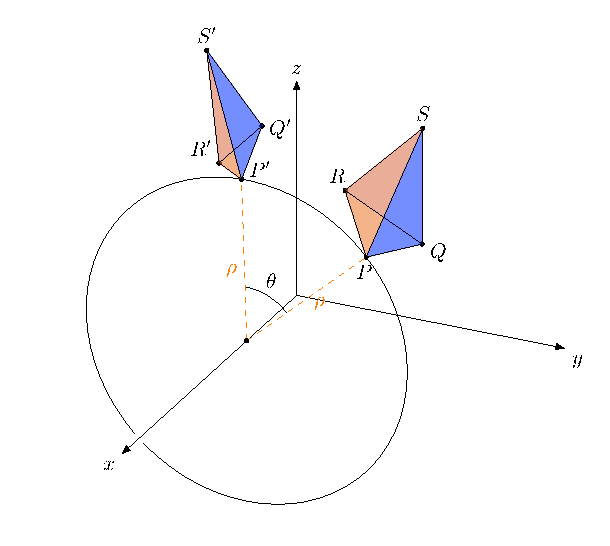
\includegraphics[scale=1]{Chapter3/pyramid-x-turn.pdf}
  \end{center}
  \caption{Στροφή ως προς άξονα $x$}
\end{figure}


\begin{figure}[hbt]
  \begin{center}
	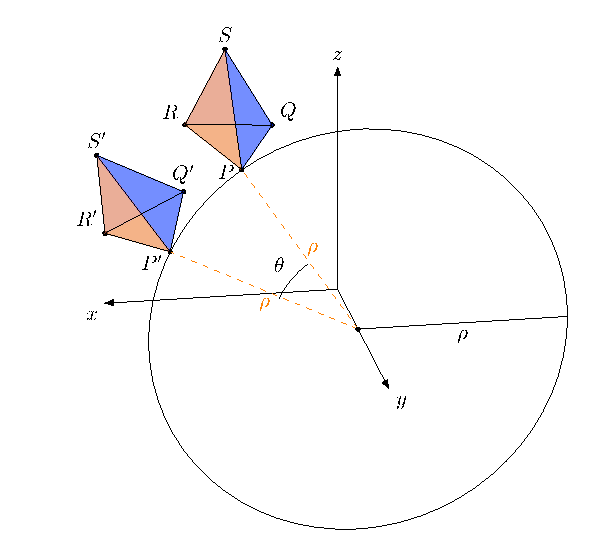
\includegraphics[scale=1]{Chapter3/pyramid-y-turn.pdf}
  \end{center}
  \caption{Στροφή ως προς άξονα $y$}
\end{figure}

\begin{figure}[hbt]
  \begin{center}
	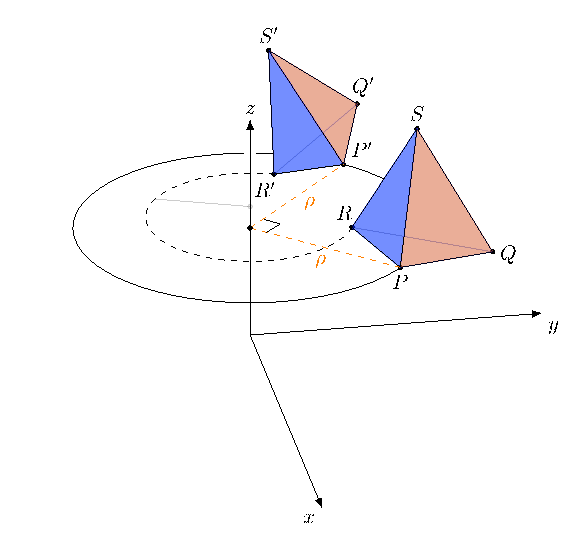
\includegraphics[scale=1]{Chapter3/pyramid-z-turn.pdf}
  \end{center}
  \caption{Στροφή ως προς άξονα $z$}
\end{figure}

% Page 73 start

%%%%%%%%%%3 

\[
R_{\theta, y} = 
\begin{bmatrix}
\cos{\theta} & 0 & \sin{\theta} & 0 \\
0 & 1 & 0 & 0 \\
-\sin{\theta} & 0 & \cos{\theta} & 0 \\
0 & 0 & 0 & 1
\end{bmatrix}
\]

\subsection{ Στροφή γύρω από τον άξονα \( x \)}

\[
P' = R_{\theta, x}(P)
\]
με
\[
x' = x, \quad y' = y \cos{\theta} - z \sin{\theta}, \quad z' = y \sin{\theta} + z \cos{\theta}
\]
και:
\[
R_{\theta, x} = 
\begin{bmatrix}
1 & 0 & 0 & 0 \\
0 & \cos \theta & -\sin \theta & 0 \\
0 & \sin \theta & \cos \theta & 0 \\
0 & 0 & 0 & 1
\end{bmatrix}
\]

\section{Συμμετρία ως προς επίπεδο}

Δίνουμε τους αντίστοιχους πίνακες μετασχηματισμών:

\[
M_{x, y} = 
\begin{bmatrix}
1 & 0 & 0 & 0 \\
0 & 1 & 0 & 0 \\
0 & 0 & -1 & 0 \\
0 & 0 & 0 & 1
\end{bmatrix}
\]

\[
M_{x, z} = 
\begin{bmatrix}
1 & 0 & 0 & 0 \\
0 & -1 & 0 & 0 \\
0 & 0 & 1 & 0 \\
0 & 0 & 0 & 1
\end{bmatrix}
\]

\[
M_{y, z} = 
\begin{bmatrix}
-1 & 0 & 0 & 0 \\
0 & 1 & 0 & 0 \\
0 & 0 & 1 & 0 \\
0 & 0 & 0 & 1
\end{bmatrix}
\]


% Page 74 start

\subsection{Αντίστροφοι μετασχηματισμοί}

Για τους αντίστροφους μετασχηματισμούς ισχύει:

\begin{align*}
	T^{-1}_{v} &= T_{-v}\\
	R^{-1}_{\theta} &= R_{-\theta}\\
	S^{-1}_{S_x,S_y,S_z} &= S_{\frac{1}{S_x}, \frac{1}{S_y}, \frac{1}{S_z}}
\end{align*}

\subsection{Μετασχηματισμοί αξόνων συντεταγμένων}

\begin{figure}[hbt]
  \begin{center}
	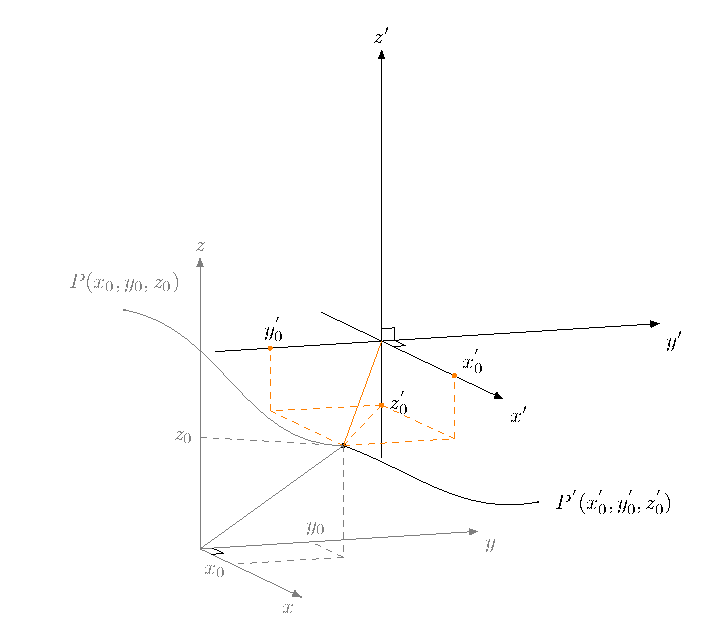
\includegraphics[scale=1]{Chapter3/axis-transformation1.pdf}
  \end{center}
  \caption{Παράλληλη μεταφοράς των αξόνων συντεταγμένων κατά διάνυσμα \( v = (t_x, t_y, t_z) \)}
\end{figure}

\begin{figure}[hbt]
  \begin{center}
	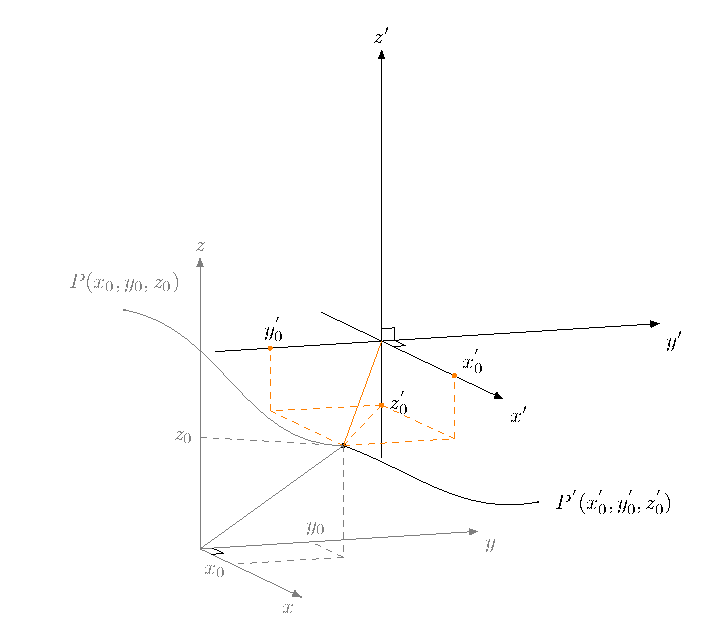
\includegraphics[scale=1]{Chapter3/axis-transformation2.pdf}
  \end{center}
  \caption{Κάτοψη: Παράλληλη μεταφοράς των αξόνων συντεταγμένων κατά διάνυσμα \( v = (t_x, t_y, t_z) \)}
\end{figure}

Στην περίπτωση της παράλληλης μεταφοράς των αξόνων συντεταγμένων κατά διάνυσμα \( v = (t_x, t_y, t_z) \) έχουμε για τις νέες συντεταγμένες \( (x', y', z') \) του σημείου \( P(x, y, z) \) θα ισχύει:

\begin{align*}
	x' &= x - t_x \\ 
	y' &= y - t_y \\
	z' &= z - t_z
\end{align*}

Άρα ο μετασχηματισμός \( \overline{T_v} \) θα είναι ο αντίστοιχος του \( T_{-v} \) γεωμετρικού μετασχηματισμού.

Αντί των πινάκων συντεταγμένων θα δώσουμε εδώ συνοπτικά τις αντιστοιχίες μεταξύ μετασχηματισμών αξόνων συντεταγμένων και γεωμετρικών.

\begin{itemize}
    \item Μεταφορά:  
    \( \overline{T_v} \longleftrightarrow T_{-v} \)

    \item Μετασχηματισμός κλίμακας:  
    \( \overline{S_{S_x,S_y,S_z}} \longleftrightarrow S_{\frac{1}{S_x}, \frac{1}{S_y}, \frac{1}{S_z}} \)

    \item Στροφή:  
    \( \overline{R_{\theta}} \longleftrightarrow R_{-\theta} \quad \)
    \( \overline{R_{\theta,x}} \longleftrightarrow R_{-\theta,x} \)

    \( \overline{R_{\theta,y}} \longleftrightarrow R_{-\theta,y} \)

    \( \overline{R_{\theta,z}} \longleftrightarrow R_{-\theta,z} \)
\end{itemize}

Για τους αντίστροφους τέλος μετασχηματισμούς αξόνων συντεταγμένων ισχύει:

\begin{align*}
	\overline{T^{-1}_{v}} &= T_{-V} \\
	\overline{R^{-1}_{\theta}} &= R_{-\theta} \\ 
	\overline{S^{-1}_{S_x,S_y,S_z}} &= S_{\frac{1}{S_x}, \frac{1}{S_y}, \frac{1}{S_z}}
\end{align*}

 
% Page 75 start

\begin{remark}
	Όπως και στην περίπτωση των δύο συντεταγμένων, έτσι και εδώ, πεπλεγμένοι μετασχηματισμοί αντιμετωπίζονται με τη διαδικασία της σύνθεσης συναρτήσεων η οποία εδώ ταυτίζεται με τον πολλαπλασιασμό πινάκων. 
\end{remark}


% Page 76 start


\section{Παραδείγματα μετασχηματισμών στο χώρο}

%%\begin{example}
%	Να προσδιορίσετε μετασχηματισμό $A_v$ που ευθυγραμμίζει $v$ με το μοναδιαίο διάνυμα $\vec{k}$ του άξονα $z$.
%\end{example}
%



\begin{example}
	Να υπολογιστεί ο πίνακας μετασχηματισμού \( T \) για την περίπτωση στροφής γύρω από τον άξονα \( x \) κατά γωνία \( \theta _x \) και στη συνέχεια στροφή ως προς \( y \) κατά γωνία \( \theta _y \).
\end{example}

\begin{solution}
	Ο μετασχηματισμός προκύπτει διαδοχικά. Αρχικά συμβαίνει στροφή γύρω από τον άξονα \( x \) κατά γωνία \( \theta _x \) και έπειτα η στροφή ως προς τον άξονα \( y \) κατά γωνία \( \theta  _y \). Θα εκμεταλλευτούμε τη διαδικάσια σύνθεσης των παραπάνω μετασχηματισμών. Αναλυτικότερα: 
\begin{align*}
	T &= R_{\theta _y, y}  \circ R_{\theta _x, x} =
		\begin{bmatrix}
		\cos \theta_y & 0 & \sin \theta_y & 0 \\
		0 & 1 & 0 & 0 \\
		-\sin \theta_y & 0 & \cos \theta_y & 0 \\
		0 & 0 & 0 & 1
		\end{bmatrix}
	\cdot	
		\begin{bmatrix}
		1 & 0 & 0 & 0 \\
		0 & \cos \theta_x & -\sin \theta_x & 0 \\
		0 & \sin \theta_x & \cos \theta_x & 0 \\
		0 & 0 & 0 & 1
		\end{bmatrix}
	= \\ 
	&=
		\begin{bmatrix}
		\cos \theta_y & \sin \theta_y \sin \theta_x & \sin \theta_y \cos \theta_x & 0 \\
		0 & \cos \theta_x & -\sin \theta_x & 0 \\
		-\sin \theta_y & \cos \theta_y \sin \theta_x & \cos \theta_y \cos \theta_x & 0 \\
		0 & 0 & 0 & 1
		\end{bmatrix}
\end{align*}

\end{solution}
\begin{example}
	Ορίζουμε ως "καμπή" την περιστροφή γύρω από τον άξονα \( x \) και στη συνέχεια γύρω από τον άξονα \( y \). 
	
	\begin{enumerate}
	    \item[i)] Βρείτε τον πίνακα καμπής \( T_k \).
  	    \item[ii)] Εξετάστε εάν παίζει ρόλο η σειρά με την οποία εκτελείται η περιστροφή.
	\end{enumerate}
\end{example}

\begin{solution}
	
\begin{enumerate}
	    \item[i)]   Τα ακόλουθα βήματα καθορίζουν τον ζητούμενο πίνακα.


\textbf{Βήμα 1:} Στροφή κατά γωνία \( \theta_x \) ως προς τον άξονα \( x \).

    Βασικός πίνακας μετασχηματισμού: \( R_{\theta_x, x} \).

\textbf{Βήμα 2:} Στροφή κατά γωνία \( \theta_y \) ως προς τον άξονα \( y \).

    Βασικός πίνακας μετασχηματισμού: \( R_{\theta_y, y} \).

    Ο ζητούμενος πίνακας θα προκύψει σαν σύνθεση των παραπάνω βασικών μετασχηματισμών.




%%%%%%%%%% 6

\begin{align*}
T_k &= R_{\theta_y, y}  \circ R_{\theta_x, x} = 
		\begin{bmatrix}
		\cos \theta_y & 0 & \sin \theta_y & 0 \\
		0 & 1 & 0 & 0 \\
		-\sin \theta_y & 0 & \cos \theta_y & 0 \\
		0 & 0 & 0 & 1
		\end{bmatrix}
	\cdot 
		\begin{bmatrix}
		1 & 0 & 0 & 0 \\
		0 & \cos \theta_x & -\sin \theta_x & 0 \\
		0 & \sin \theta_x & \cos \theta_x & 0 \\
		0 & 0 & 0 & 1
		\end{bmatrix} = \\
	&= 
		\begin{bmatrix}
		\cos \theta_y & \sin \theta_y \sin \theta_x & \sin \theta_y \cos \theta_x & 0 \\
		0 & \cos \theta_x & -\sin \theta_x & 0 \\
		-\sin \theta_y & \cos \theta_y \sin \theta_x & \cos \theta_y \cos \theta_x & 0 \\
		0 & 0 & 0 & 1
		\end{bmatrix}
\end{align*}

	    \item[ii)]  Εάν εκτελεστούν οι παραπάνω μετασχηματισμοί με αντίθετη σειρά θα προκύψει ο ακόλουθος πίνακας:

\[
T_k = R_{\theta_x, x} \cdot R_{\theta_y, y} = 
	\begin{bmatrix}
	\cos \theta_y & 0 & \sin \theta_y & 0 \\
	\sin \theta_x \sin \theta_y & \cos \theta_x & -\sin \theta_x \cos \theta_y & 0 \\
	-\cos \theta_x \sin \theta_y & \sin \theta_x & \cos \theta_x \cos \theta_y & 0 \\
	0 & 0 & 0 & 1
	\end{bmatrix}
\]	

Παρατηρούμε ότι ο νέος πίνακας διαφέρει από αυτόν του ερωτήματος (i) επομένως παίζει σημαντικό ρόλο η σειρά με την οποία εκτελείται η περιστροφή.

\end{enumerate}

\end{solution}
\begin{example}
Προσδιορίστε το μετασχηματισμό $M$ που περιστρέφει τη δοσμένη πυραμίδα $ABCD$ κατά γωνία $\theta$ ως προς το δοσμένο άξονα περιστροφής $R$.

		\begin{figure}[hbt]
		\begin{center}
		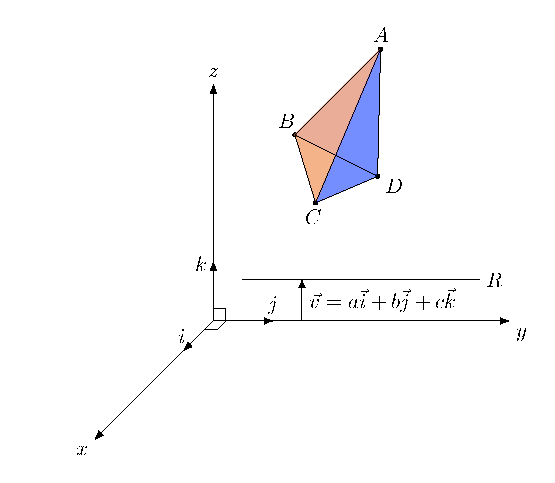
\includegraphics[scale=1]{Chapter3/example-pyramid.pdf}
		\end{center}
		\caption{Πυραμίδα $ABCD$ που ζητείται να περιστραφεί κατά γωνία $\theta$ ως προς το δοσμένο άξονα περιστροφής $R$}
		\end{figure}

\end{example}

\begin{solution}
	Παρατηρούμε ότι ο άξονας $R$ είναι παράλληλος ως προς το επίπεδο $xz$ και βρίσκεται σε απόσταση που καθορίζεται από το διάνυσμα $v$. Θα προσπαθήσουμε λοιπόν να τον ταυτίσουμε με τον άξονα των $x$. Τα ακόλουθα βήαμτα χρειάζονται για να προσδιορίσουμε τον ζητούμενο πίνακα μετασχηματισμού.

\textbf{Βήμα 1:} Μεταφορά του $R$ κατά διάνυμσα $v = -a\vec{i} - b\vec{j} - c\vec{k}$ ώστε ο άξονας περιστροφής να συμπέσει με τον άξονα των $x$

Βασικός πίνακας μετασχηματισμού $T_v$.

\textbf{Βήμα 2:} Στροφή ως προς τον άξονα των $x$ κατά γωνία $\theta$. 

Βασικός πίνακας μετασχηματισμού $R_{\theta, x}$.
 
\textbf{Βήμα 3:} Επαναφορά του $R_{-v}$ στην αρχική του θέση μεταφέροντας τον κατά διάνυσμα $-v$.

Βασικός πίνακας μετασχηματισμού $T_{-v}$.

Ο ζητούμενος μετασχηματισμός $M$ προκύπτει σα σύνθεση των παραπάνω βασικών μετασχηματισμών:

\begin{align*}
	M & = T_{-v} \circ R_{\theta, x} \circ T_v 	= 
		\begin{bmatrix}
			1 & 0 & 0 & a \\
			0 & 1 & 0 & b \\
			0 & 0 & 1 & c \\
			0 & 0 & 0 & 1
		\end{bmatrix} 
	\cdot 
		\begin{bmatrix}
			1 & 0 & 0 & 0 \\
			0 & \cos{\theta} & -\sin{\theta} & 0 \\
			0 & \sin{\theta} & \cos{\theta} & 0 \\
			0 & 0 & 0 & 1
		\end{bmatrix}
	\cdot 
		\begin{bmatrix}
			1 & 0 & 0 & -a \\
			0 & 1 & 0 & -b \\
			0 & 0 & 1 & -c \\
			0 & 0 & 0 & 1
		\end{bmatrix}  = \\
	&=	
	\begin{bmatrix}
			1 & 0 & 0 & 0 \\
			0 & \cos{\theta} & -\sin{\theta} & -b\cos{\theta} + c\sin{\theta} + b \\
			0 & \sin{\theta} & \cos{\theta} & -b\sin{\theta}-c\cos{\theta} + c \\
			0 & 0 & 0 & 1
		\end{bmatrix}  
\end{align*}

		Οι συντεταγμένες $A'B'C'D'$ της στραμμένης πυραμίδας προκύπτουν από τον ακόλουθο πολλαπλασιασμό: 
		
\[
	A'B'C'D' = M \cdot ABCD
\]		
	
\begin{remark}
	Είναι ιδιαιτέρως χρήσιμο στους μετασχηματισμούς στο χώρο των τριών διαστάσεων να μπορέσουμε να καθορίσουμε τον πίνακα μετασχηματισμού που εκφράζει τη στροφή ενός αντικειμένου ως προς ένα οποιοδήποτε δοσμένο άξονα στον χώρο. Στα επόμενα παραδείγματα αντιμετωπίζεται το συγκεκριμένο πρόβλημα.	
\end{remark}

	
\end{solution}
\begin{example}
Προσδιορίστε το μετασχηματισμό $A_v$ που ευθυγραμμίζει δοσμένο διάνυσμα $\vec{v}$ με το μοναδιαίο διάνυσμα $\vec{k}$ κατά μήκος του θετικού μέρους του άξονα των $z$.

\end{example}

\begin{solution}
	Τα ακόλουθα βήματα απαιτούνται για το ζητούμενο μετασχηματισμό. 
	
\textbf{Βήμα 1:} Περιστροφή του διανύσματος $v$ γύρω από τον άξονα $x$ κατά γωνία $\theta_1$ έτσι ώστε το $v$ να πέφτει στο πάνω μέρος του επιπέδου $xz$ (διάνυσμα $v_1$, Σχήμα \ref{fig:10}

\begin{center}
	Βασικός πίνακας μετασχηματισμού $R_{\theta_1, x}$.
\end{center}

\textbf{Βήμα 2:} Περιστροφή του διανύσματος $v_1$ γύρω από τον άξονα των $y$ κατά γωνία $-\theta_2$ έτσι ώστε ώστε το $v_1$ να πέσει πάνω στο θετικό μέρος του άξονα των $z$ (διάνυσμα $v_2$ Σχήμα \ref{fig:11}).

\begin{center}
	Βασικός πίνακας μετασχηματισμού $R_{-\theta_2, x}$.
\end{center}


\begin{figure}[h!]
	\begin{center}
		\begin{minipage}[b]{0.48\textwidth} % Top-left image
		%    \centering
		    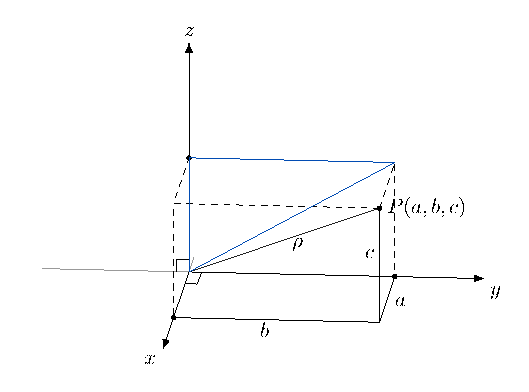
\includegraphics[scale=1]{Chapter3/Av1.pdf}
%		    \captionof{figure}{}
		\end{minipage}%
	\hfill
		\begin{minipage}[b]{0.48\textwidth} % Top-right image
		%    \centering
		    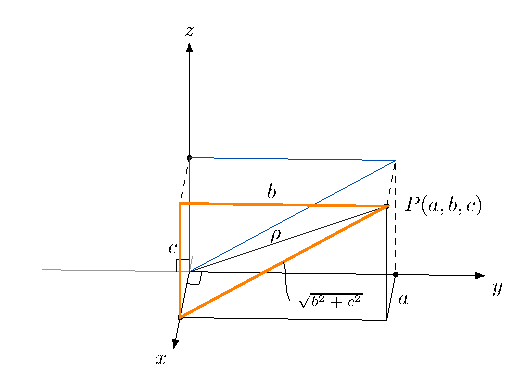
\includegraphics[scale=1]{Chapter3/Av2.pdf}
%		    \captionof{figure}{Βήμα 4}
		\end{minipage}
	\end{center}
	\caption{Διάνυσμα $v$ που καλούμαστε να ευθυγραμμίσουμε με το μοναδιαίο διάνυμα $\vec{k}$ του άξονα $z$}
\end{figure}


\begin{figure}[h!]
	\begin{center}
		\begin{minipage}[b]{0.48\textwidth} % Top-left image
		%    \centering
		    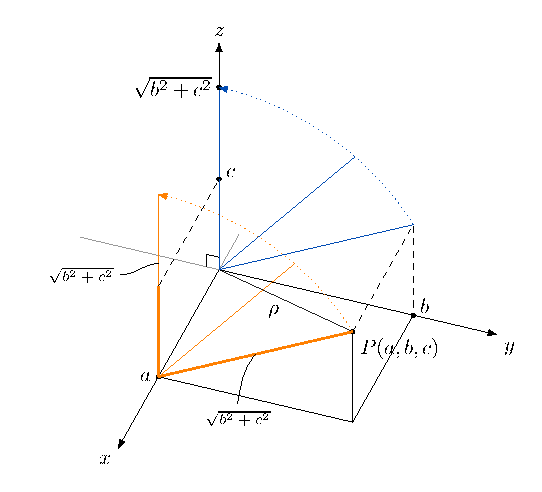
\includegraphics[scale=1]{Chapter3/Av3.pdf}
%		    \captionof{figure}{}
		\end{minipage}%
	\hfill
		\begin{minipage}[b]{0.48\textwidth} % Top-right image
		%    \centering
		    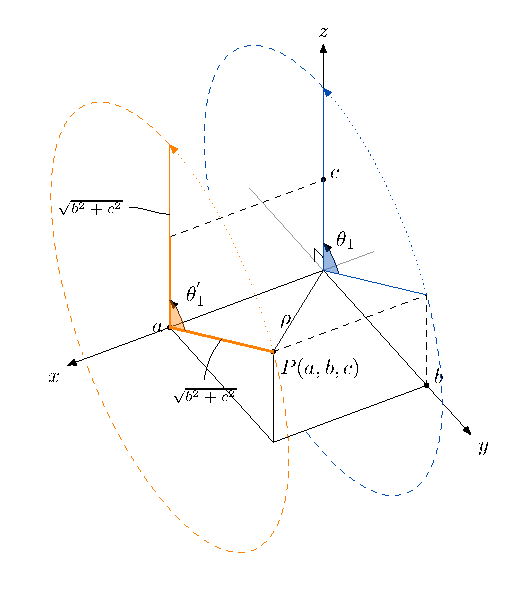
\includegraphics[scale=1]{Chapter3/Av4.pdf}
%		    \captionof{figure}{Βήμα 4}
		\end{minipage}
	\end{center}
	\caption{Βήμα 1: Περιστροφή του διανύσματος $v$ γύρω από τον άξονα $x$ κατά γωνία $\theta_1$ έτσι ώστε το $v$ να πέσει στο επίπεδο $xz$}
\end{figure}


\begin{figure}[h!]
	\begin{center}
%		\begin{minipage}[b]{0.48\textwidth} % Top-left image
		%    \centering
		    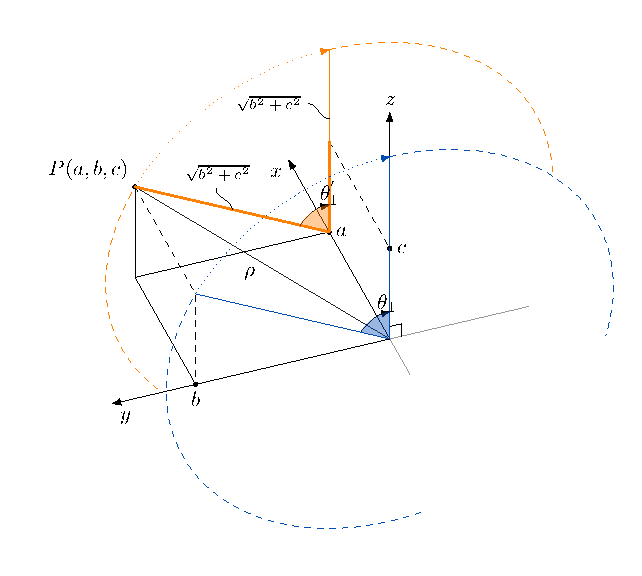
\includegraphics[scale=0.8]{Chapter3/Av4-reverse.pdf}
%		    \captionof{figure}{}
%		\end{minipage}%
	\end{center}
	\caption{Διαφορετική όψη στροφής διανύσματος $v$ γύρω από τον άξονα $x$}		
\end{figure}


\begin{figure}[h!]
	\begin{center}
		\begin{minipage}[b]{0.48\textwidth} % Top-left image
		%    \centering
		    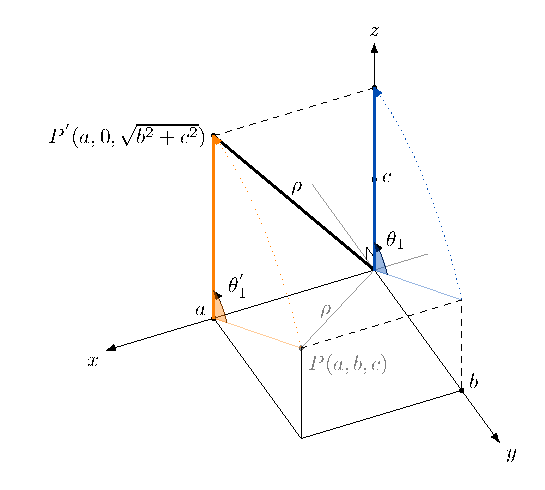
\includegraphics[scale=1]{Chapter3/Av5.pdf}
%		    \captionof{figure}{}
		\end{minipage}%
	\hfill
		\begin{minipage}[b]{0.48\textwidth} % Top-right image
		%    \centering
		    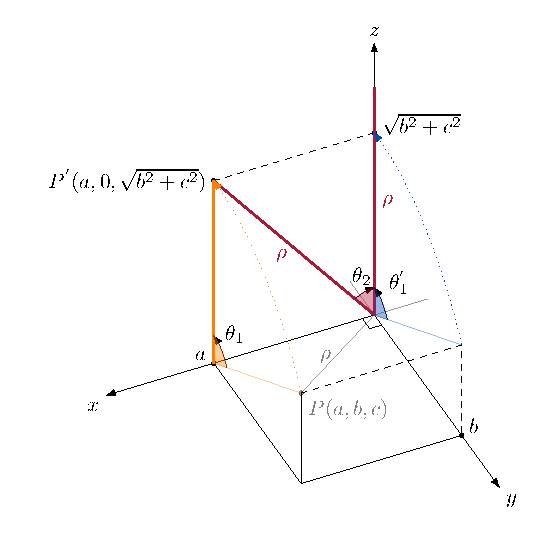
\includegraphics[scale=1]{Chapter3/Av6.pdf}
%		    \captionof{figure}{Βήμα 4}
		\end{minipage}
	\end{center}
	\caption{Βήμα 2: Περιστροφή του διανύσματος $v_1$ γύρω από τον άξονα των $y$ κατά γωνία $-\theta_2$ έτσι ώστε ώστε το $v_1$ να πέσει πάνω στο θετικό μέρος του άξονα των $z$}
\end{figure}

Ο ζητούμενος πίνακας θα προκύψει σαν σύνθεση των παραπάνω βασικών μετασχηματισμών αφού όμως πρώτα προσδιοριστούν οι γωνίες $\theta_1$ και $\theta_2$.

\underline{Προσδιορισμός των γωνιών $\theta_1$ και $\theta_2$:} Από το Σχήμα  \ref{fig:11} παρατηρούμε ότι η ζητούμενη γωνία $\theta_1$ θα προσδιοριστεί από τη γωνία που σχηματίζει η προβολή του $v$ στο επίπεδο $yz$ με τον άξονα των $z$. (υποθέτουμε ότι $b$ και $c$ δεν είναι και τα δύο μηδέν). Από το τρίγωνο $OP'B$ \textcolor{red}{check} προκύπτει:

\begin{align*}
	\sin{\theta_1} &= \cfrac{b}{\sqrt{b^2 + c^2}} \\
	\cos{\theta_1} &= \cfrac{c}{\sqrt{b^2 + c^2}}
\end{align*}


Ο πίνακας περιστροφής \(R_{\theta_1, x}\) ισούται με:

\[
R_{\theta_1, x} =
\begin{bmatrix}
1 & 0 & 0 & 0\\
0 & \cfrac{c}{\sqrt{b^2 + c^2}} & \cfrac{-b}{\sqrt{b^2 + c^2}} & 0\\
0 & \cfrac{b}{\sqrt{b^2 + c^2}} & \cfrac{c}{\sqrt{b^2 + c^2}} & 0 \\
0 & 0 & 0 & 1
\end{bmatrix}
\]

Επιδρώντας με αυτόν τον πίνακα στο διάνυσμα $v(a, b, c)$ προκύπτουν οι συντεταγμένες του $v_1(x, y, z)$:

\[
		\begin{bmatrix}
			x \\
			y \\
			z \\
			1
		\end{bmatrix}
	=
		R_{\theta_1, x} \cdot 
		\begin{bmatrix}
			a \\
			b \\
			c \\ 
			1
		\end{bmatrix}
	= 
		\begin{bmatrix}
			1 & 0 & 0 & 0\\
			0 & \cfrac{c}{\sqrt{b^2 + c^2}} & \cfrac{-b}{\sqrt{b^2 + c^2}} & 0\\
			0 & \cfrac{b}{\sqrt{b^2 + c^2}} & \cfrac{c}{\sqrt{b^2 + c^2}} & 0 \\
			0 & 0 & 0 & 1
		\end{bmatrix}
	\cdot 
		\begin{bmatrix}
			a \\
			b \\
			c \\ 
			1
		\end{bmatrix}
	=
		\begin{bmatrix}
			a \\
			0 \\
			\sqrt{b^2+c^2} \\ 
			1
		\end{bmatrix}
\]

Για τον προσδιορισμό της γωνίας $\theta_2$ από το τρίγωνο $OQQ'$ (Σχήμα \ref{fig:11}) προκύπτει:

\begin{align*}
	\sin{(-\theta_2)} &= = -\sin{\theta_2} -\cfrac{a}{\sqrt{a^2 + b^2 + c^2}} \\	
	\cos{(-\theta_2)} &= \cos{\theta_2} = \cfrac{\sqrt{b^2 + c^2}}{\sqrt{a^2 + b^2 + c^2}}
\end{align*}

Τελικά, ο ζητούμενος μετασχηματισμός $A_v$ θα ισούται με:

\[
	A_v = R_{-\theta_2, y} \cdot R_{\theta_1, x}
\]

Αντικαθιστώντας τις προηγούμενες γωνίες στους πίνακες $R_{-\theta_2, y}, R_{\theta_1, x}$ και θέτοντας $\lambda = \sqrt{b^2 + c^2}$, προκύπτει:

\[
	A_v =
	\begin{bmatrix}
		\cfrac{\lambda}{|v|} & \cfrac{-ab}{\lambda |v|} & \cfrac{-ac}{\lambda |v|} & 0 \\
		0 & \cfrac{c}{\lambda} & \cfrac{-b}{\lambda} & 0 \\
		\cfrac{a}{|v|} & \cfrac{b}{|v|} & \cfrac{c}{|v|} & 0 \\
		0 & 0 & 0 & 1
	\end{bmatrix}, \ \text{όπου} \ |v| = \sqrt{a^2 + b^2 + c^2}
\]


\begin{remark}
	Εάν \(b\) και \(c\) ισούνται με μηδέν, τότε \(\lambda = 0\). Σε αυτή την περίπτωση απαιτείται μόνο μία περιστροφή \(90^\circ\) ως προς τον άξονα των \(y\). Τότε $v= a\vec{i}$, δηλαδή το δοσμένο διάνυσμα βρίσκεται επί του άξονα $x$. Δηλαδή:

	\[
		A_v = R_{-\theta_2, y} =
		\begin{bmatrix}
			0 & 0 & \cfrac{-a}{|a|} & 0 \\
			0 & 1 & 0 & 0 \\
			\cfrac{a}{|a|} & 0 & 0 & 0 \\
			0 & 0 & 0 & 1
		\end{bmatrix}
	\]
\end{remark}


\begin{remark}	
	Με τον ίδιο τρόπο μπορούμε να υπολογίσουμε τον αντίστροφο μετασχηματισμό \(A_v^{-1}\), που ευθυγραμμίζει το μοναδιαίο διάνυσμα \(\vec{k}\) με το δοσμένο διάνυσμα \(v\). Πιο συγκεκριμένα:
	
	\[
	A_v^{-1} 
		= \left(R_{-\theta_2, y} \cdot R_{\theta_1, x}\right)^{-1} 
		= R_{\theta_1, x}^{-1} \cdot R_{-\theta_2, y}^{-1}
		= R_{-\theta_1, x} \cdot R_{\theta_2, y} 
		= 	\begin{bmatrix}
				\cfrac{\lambda}{|v|} & 0 & \cfrac{a}{|v|} & 0 \\
				\cfrac{-ab}{\lambda |v|} & \cfrac{c}{\lambda} & \cfrac{b}{|v|} & 0 \\
				\cfrac{-ac}{\lambda|v|} & \cfrac{-b}{\lambda} & \cfrac{c}{|v|} & 0 \\
				0 & 0 & 0 & 1
			\end{bmatrix}
	\]
\end{remark}


\begin{remark}	
	Με τη βοήθεια του μετασχηματισμού \(A_v\) μπορούμε να ταυτίσουμε οποιονδήποτε δοσμένο άξονα στον χώρο με κάποιον από τους \(O_x, O_y, O_z\). Έτσι μπορούμε να ανάγουμε το πρόβλημα της στροφής ως προς ένα οποιοδήποτε άξονα \(R\) του χώρου σε πρόβλημα στροφής ως προς τον άξονα \(O_x, O_y\) ή \(O_z\) με τον οποίο θα έχουμε ταυτίσει τον \(R\).  
\end{remark}

	
\end{solution}
\begin{example}
Βρείτε το μετασχηματισμό που περιστρέφει δοσμένο σημείο \(Q\) ως προς άξονα περιστροφής \(L\) που περνάει από ένα καθορισμένο σημείο \(P\) και η διεύθυνσή του καθορίζεται από επίσης δοσμένο διάνυσμα \(v\).  	
\end{example}

\begin{solution}
	
\end{solution}

\begin{example}
 Βρείτε το συμμετρικό του πολυγώνου $V$ με κορυφές $A(-1, 0)$, $B(0, -2)$, $C(1, 0)$ και $D(0, 2)$ ως προς:
\begin{enumerate}
    \item[α)] οριζόντια ευθεία $y=2$
    \item[β)] κατακόρυφη ευθεία $x=2$
    \item[γ)] ευθεία $y=x+2$
\end{enumerate}
\end{example}


\begin{solution}
Το πολύγωνο παρουσιάζεται υπό μορφή πίνακα ως εξής:

\[
V = \begin{bmatrix}
-1 & 0 & 1 & 0 \\
0 & -2 & 0 & 2 \\
1 & 1 & 1 & 1
\end{bmatrix}
\]

Θα χρησιμοποιήσουμε τον πίνακα $M_L$ όπως έχει ορισθεί στο Παράδειγμα 5.\\
α) Η ευθεία $y=2$ έχει σημείο τομής με τον άξονα των $y$ το $(0,2)$ και σχηματίζει γωνία $\theta = 0$ με τον $x$. Επομένως $\theta=0$, $m=0$ και $v=2\hat{j}$. Αντικαθιστώντας αυτές τις τιμές στον πίνακα $M_l$ προκύπτει:
    \[
    M_L = \begin{bmatrix}
    1 & 0 & 0 \\
    0 & -1 & 4 \\
    0 & 0 & 1
    \end{bmatrix}
    \]
Αυτός ο πίνακας αναστρέφει το πολύγωνο συμμετρικά ως προς $y=2$.
Οι συντεταγμένες του καινούργιου πολυγώνου προκύπτουν από τη σχέση:

\[
V' = A'B'C'D' = M_L \cdot V = \begin{bmatrix}
1 & 0 & 0 \\
0 & -1 & 4 \\
0 & 0 & 1
\end{bmatrix}
\begin{bmatrix}
-1 & 0 & 1 & 0 \\
0 & -2 & 0 & 2 \\
1 & 1 & 1 & 1
\end{bmatrix}
= \begin{bmatrix}
-1 & 0 & 1 & 0 \\
4 & 6 & 4 & 2 \\
1 & 1 & 1 & 1
\end{bmatrix}
\]

Τελικό $A' = (-1, 4)$, $B' = (0, 6)$, $C' = (1, 4)$ και $D' = (0, 2)$.

β) Η ευθεία $x=2$ (Σχήμα ) είναι παράλληλη με τον άξονα των $y$ άρα δεν έχει σημείο τομής. Επίσης, έχει άπειρη κλίση! Γι' αυτό αν $v = 2\hat{i}$ θα πρέπει να εκτελεστεί ο ακόλουθος μετασχηματισμός:\\
Βήμα 1: Μεταφορά κατά διάνυσμα $-v$, ώστε η ευθεία $x=2$ να πάει πάνω στον άξονα $y$.
\[
\text{Βασικός πίνακας μετασχηματισμού: } T_{-v}
\]
Βήμα 2: Συμμετρία ως προς $y$.
\[
\text{Βασικός πίνακας μετασχηματισμού: } M_y
\]
Βήμα 3: Επαναφορά της ευθείας $x=2$ στην αρχική της θέση, δηλαδή μεταφορά κατά διάνυσμα $v$.
\[
\text{Βασικός πίνακας μετασχηματισμού: } T_v
\]

Ο ζητούμενος μετασχηματισμός $M$ προκύπτει σαν σύνθεση των παραπάνω, δηλαδή:

\[
M = T_v \cdot M_y \cdot T_{-v} = \begin{bmatrix}
1 & 0 & 2 \\
0 & 1 & 0 \\
0 & 0 & 1
\end{bmatrix}
\begin{bmatrix}
1 & 0 & 0 \\
0 & -1 & 0 \\
0 & 0 & 1
\end{bmatrix}
\begin{bmatrix}
1 & 0 & -2 \\
0 & 1 & 0 \\
0 & 0 & 1
\end{bmatrix} = \begin{bmatrix}
1 & 0 & 0 \\
0 & -1 & 0 \\
0 & 0 & 1
\end{bmatrix}
\]

Οι συντεταγμένες του καινούργιου πολυγώνου δίνονται από:
\[
V' = A'B'C'D' = MV = \begin{bmatrix}
1 & 0 & 0 \\
0 & -1 & 0 \\
0 & 0 & 1
\end{bmatrix}
\begin{bmatrix}
-1 & 0 & 1 & 0 \\
0 & 2 & 0 & 2 \\
1 & 1 & 1 & 1
\end{bmatrix} = \begin{bmatrix}
-1 & 0 & 1 & 0 \\
0 & -2 & 0 & -2 \\
1 & 1 & 1 & 1
\end{bmatrix}
\]

Τελικό $A' = (-1, 0)$, $B' = (0, -2)$, $C' = (1, 0)$ και $D' = (0, -2)$.

γ) Η ευθεία $y=x+2$ έχει κλίση $m=1$ και σημείο τομής με τον άξονα των $y$ το $(0,2)$, επομένως $b=2$. Ο πίνακας $M_l$ του παραδείγματος 5 παίρνει την ακόλουθη τιμή:
\[
M_l = \begin{bmatrix}
0 & 1 & -2 \\
1 & 0 & 2 \\
0 & 0 & 1
\end{bmatrix}
\]

Οι συντεταγμένες του καινούργιου πολυγώνου δίνονται από:
\[
V' = A'B'C'D' = M_l V = \begin{bmatrix}
0 & 1 & -2 \\
1 & 0 & 2 \\
0 & 0 & 1
\end{bmatrix}
\begin{bmatrix}
-1 & 0 & 1 & 0 \\
0 & 2 & 0 & 2 \\
1 & 1 & 1 & 1
\end{bmatrix} = \begin{bmatrix}
2 & 2 & 0 & 2 \\
-1 & 0 & -2 & 0 \\
1 & 1 & 1 & 1
\end{bmatrix}
\]

Τελικό $A' = (2, -1)$, $B' = (2, 0)$, $C' = (0, -2)$ και $D' = (2, 0)$.

Μια στρέβλωση (shearing) κατά μήκος του $X$-άξονα, του σημείου $\overline{P}(x, y)$ με παράγοντα στρέβλωσης $a$, φέρνει το σημείο $\overline{P}$ στο $\overline{P'}(x', y')$ και ισχύει:
\[
x' = x + ay, \quad y' = y .
\]

Χρησιμοποιώντας πίνακες γράφουμε:
\[
\begin{bmatrix}
x' \\
y'
\end{bmatrix} = \begin{bmatrix}
1 & a \\
0 & 1
\end{bmatrix}
\begin{bmatrix}
x \\
y
\end{bmatrix}
\]

ή \(\overline{P'} = SH_x \cdot \overline{P}\) με:
\[
SH_x = \begin{bmatrix}
1 & a \\
0 & 1
\end{bmatrix}
\]

Για την περίπτωση της στρέβλωσης κατά μήκος του $Y$-άξονα και με παράγοντα στρέβλωσης $b$ ισχύει:
\[
SH_y = \begin{bmatrix}
1 & 0 \\
b & 1
\end{bmatrix}
\]


Στο σχήμα  δείχνεται η στρέβλωση ενός τετραγώνου για τις δύο περιπτώσεις $a=2$ και $b=2$.

\begin{figure}[h!]
	\begin{center}
		\begin{minipage}[b]{0.19\textwidth} % Top-left image
		    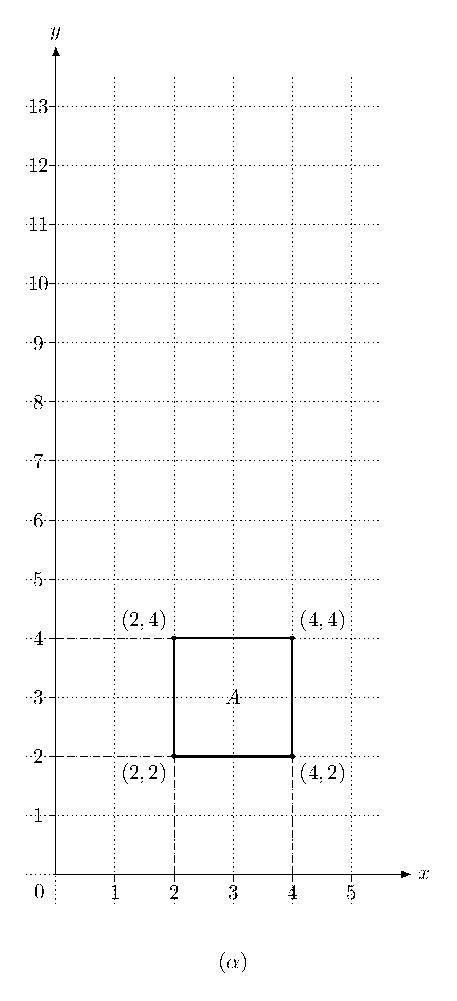
\includegraphics[width=\textwidth]{Chapter2/figure17a.pdf}
		\end{minipage}%
	\hfill
		\begin{minipage}[b]{0.4\textwidth} % Top-right image
		    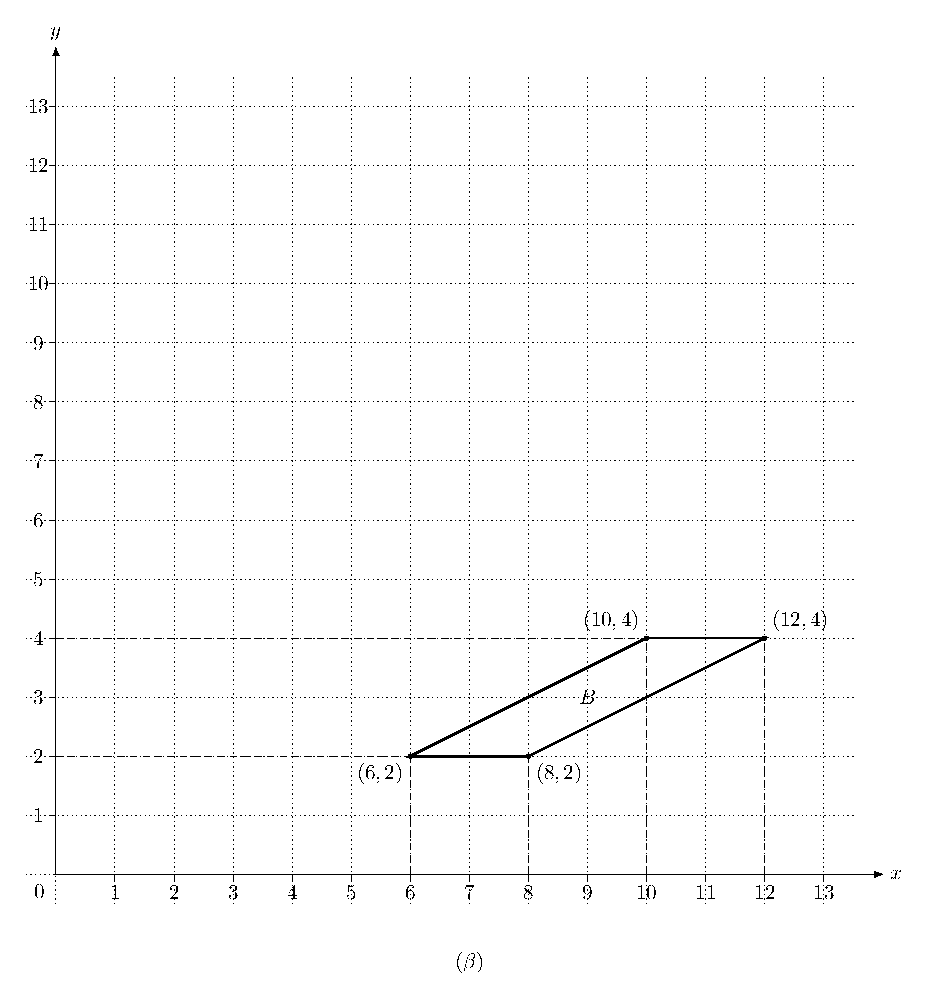
\includegraphics[width=\textwidth]{Chapter2/figure17b.pdf}
		\end{minipage}
	\hfill
		\begin{minipage}[b]{0.4\textwidth} % Top-right image
		    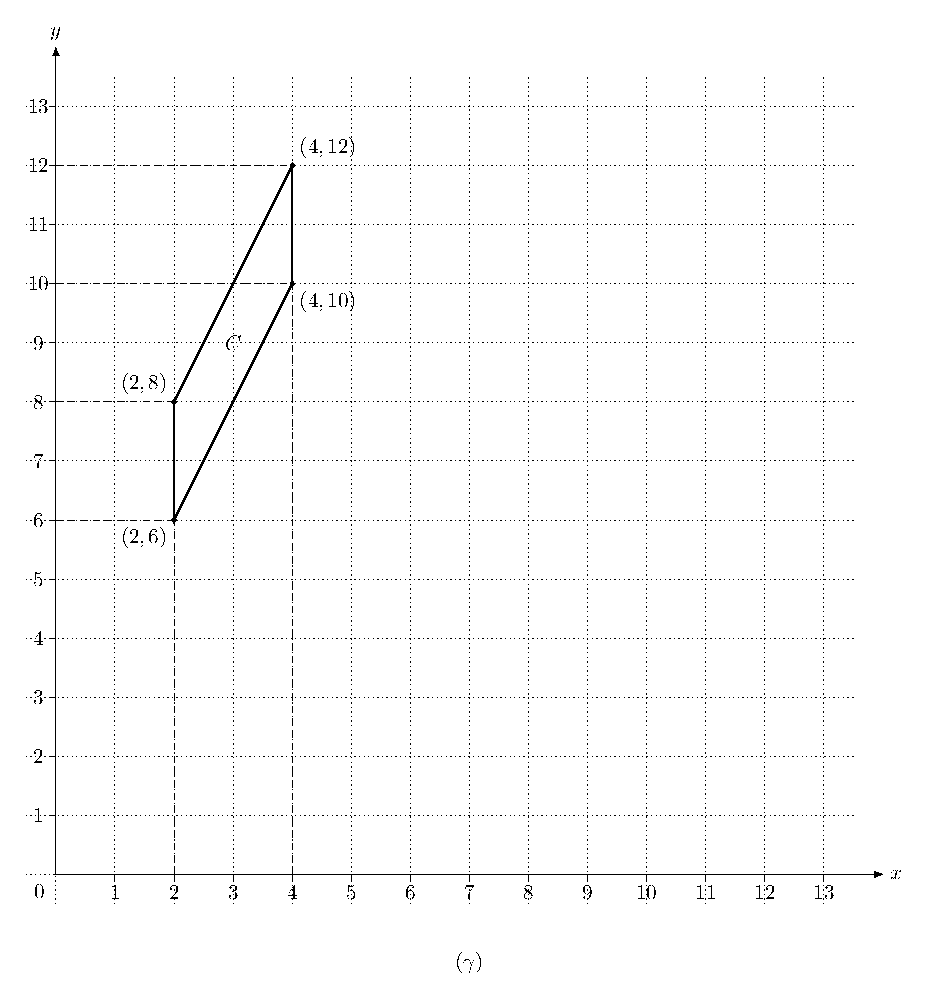
\includegraphics[width=\textwidth]{Chapter2/figure17c.pdf}
		\end{minipage}
	\end{center}
\caption{Στρέβλωση ενός τετραγώνου για $a=2$ και $b=2$}
\end{figure}

\end{solution}







\section*{Ασκήσεις 3ου Κεφαλαίου}

\begin{exercise}
Με ποια σύνθεση μετασχηματισμών μπορεί να φέρουμε την εικόνα (α), (β) στη θέση (γ).

\begin{figure}[h!]
\begin{center}
	\begin{minipage}[b]{0.3\textwidth} 
	    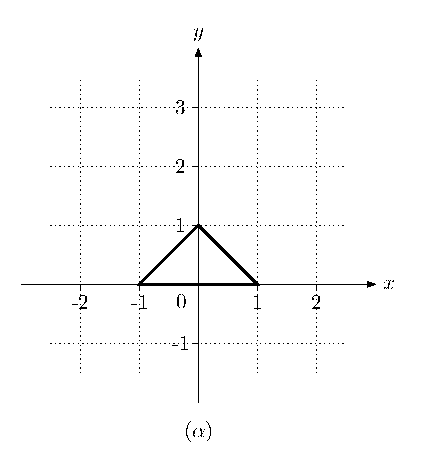
\includegraphics[width=\textwidth]{Chapter2/figure18a.pdf}
	\end{minipage}
\hfill
	\begin{minipage}[b]{0.3\textwidth} 
	    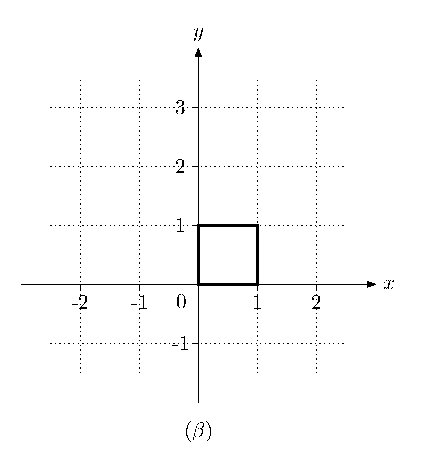
\includegraphics[width=\textwidth]{Chapter2/figure18b.pdf}
	\end{minipage}
\hfill
	\begin{minipage}[b]{0.3\textwidth} 
	    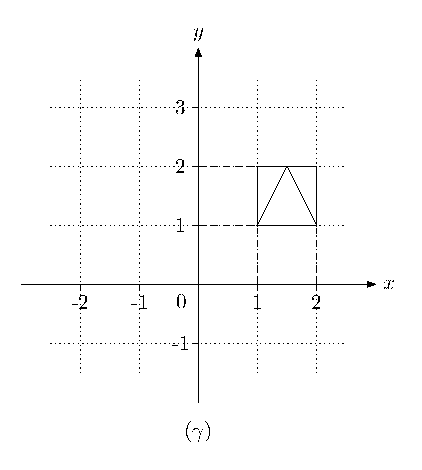
\includegraphics[width=\textwidth]{Chapter2/figure18c.pdf}
	\end{minipage}
\end{center}
\end{figure}

\end{exercise}

\begin{solution}
Πρώτα στην εικόνα (α) μπορούμε να δράσουμε ως εξής:
\begin{enumerate}
    \item Σύμπτυξη στις $x$-συντεταγμένες με: \(s_x = \cfrac{1}{2}\), \(s_y = 1\) (ως προς την αρχή των αξόνων).
    \item Μεταφορά κατά \(\vec{v} = (\cfrac{3}{2},1) \).
\end{enumerate}

Έτσι, παίρνουμε τον πίνακα μετασχηματισμού:
\[
M_{(a)} = T_v \cdot S_{\cfrac{1}{2},1} = \begin{bmatrix}
1 & 0 & \cfrac{3}{2} \\
0 & 1 & 1 \\
0 & 0 & 1
\end{bmatrix}
\begin{bmatrix}
\cfrac{1}{2} & 0 & 0 \\
0 & 1 & 0 \\
0 & 0 & 1
\end{bmatrix} = \begin{bmatrix}
\cfrac{1}{2} & 0 & \cfrac{3}{2} \\
0 & 1 & 1 \\
0 & 0 & 1
\end{bmatrix}
\]

Πράξεις:
\[
\begin{bmatrix}
\cfrac{1}{2} & 0 & \cfrac{3}{2} \\
0 & 1 & 1 \\
0 & 0 & 1
\end{bmatrix}
\begin{bmatrix}
-1 & 1 & 0 \\
0 & 0 & 1 \\
1 & 1 & 1
\end{bmatrix} = \begin{bmatrix}
1 & 2 & \cfrac{3}{2} \\
1 & 1 & 2 \\
1 & 1 & 1
\end{bmatrix}
\]


Αν στην εικόνα (β) μεταφερθεί κατά \(\vec{v} = (1,1)\), θα πάρουμε το τετράγωνο της εικόνας (γ):
\[
\begin{bmatrix}
1 & 0 & 1 \\
0 & 1 & 1 \\
0 & 0 & 1
\end{bmatrix}
\begin{bmatrix}
0 & 1 & 1 & 0 \\
1 & 0 & 1 & 1 \\
1 & 1 & 1 & 1
\end{bmatrix} = \begin{bmatrix}
1 & 2 & 2 & 1 \\
2 & 1 & 2 & 2 \\
1 & 1 & 1 & 1
\end{bmatrix}
\]

\end{solution}

\begin{exercise}
		Να προσδιοριστούν:
	\begin{enumerate}
	  \item ο πίνακας $R_{\theta, y}$ και
	  \item ο πίνακας $R_{\theta, x}$.
	\end{enumerate}
\end{exercise}

\begin{solution}
\begin{enumerate}
	
\item  Επιλέγω αρχικά σημείο που να ανήκει στο Επίπεδο $xz$.
	
		Από το σχήμα προκύπτει ότι: 
		\begin{align*}
		x' &= x\cos{\theta} + z\sin{\theta}	\\
		y' &= y \\
		z' &= -x\sin{\theta} + z\cos{\theta}	
		\end{align*}
		
		Συνεπώς:
		
		\[
		R_{\theta, y}= 
		\begin{bmatrix}
		\cos{\theta} & 0 & \sin{\theta} & 0 \\
		0 & 1 & 0 & 0 \\
		-\sin{\theta} & 0 & \cos{\theta} & 0 \\
		0 & 0 & 0 & 1
		\end{bmatrix} 
		\]	
		
		\begin{figure}[hbt]
		\begin{center}
		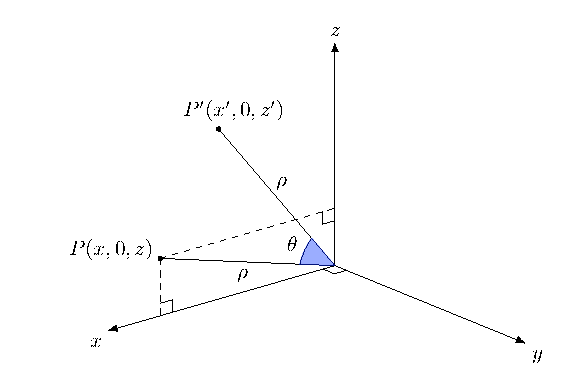
\includegraphics[scale=1]{Chapter3/point-in-xz-rotation.pdf}
		\end{center}
		\caption{Στροφή σημείου στο επίπεδο $xz$}
		\end{figure}

	
\item  Επιλέγω αρχικά σημείο που να ανήκει στο Επίπεδο $yz$.
	
		Από το σχήμα προκύπτει ότι: 
		\begin{align*}
		x' &= x \\
		y' &= y\cos{\theta} - z\sin{\theta}	\\
		z' &= y\sin{\theta} + z\cos{\theta}	
		\end{align*}
		
		Συνεπώς:
		
		\[
		R_{\theta, y}= 
		\begin{bmatrix}
		1 & 0 & 0 & 0 \\
		0 & \cos{\theta} & -\sin{\theta} & 0 \\
		0 & \sin{\theta} & \cos{\theta} & 0 \\
		0 & 0 & 0 & 1
		\end{bmatrix} 
		\]	
		
		\begin{figure}[hbt]
		\begin{center}
		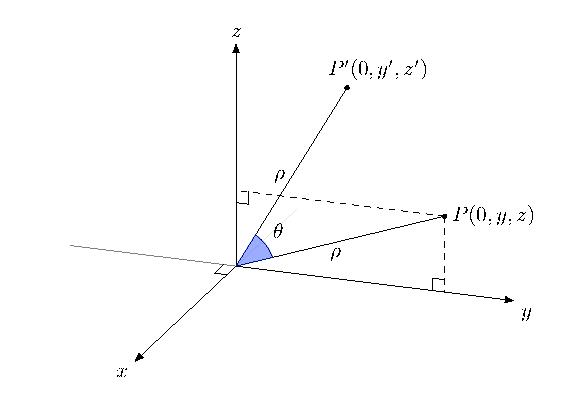
\includegraphics[scale=1]{Chapter3/point-in-yz-rotation.pdf}
		\end{center}
		\caption{Στροφή σημείου στο επίπεδο $xz$}
		\end{figure}
		
\end{enumerate}		
\end{solution}
\begin{exercise}
	Να γίνει η περιστροφή της πυραμίδας $A, B, C, D$ \textcolor{red}{which} από τον άξονα $x$ κατά $\theta_x = \ang{60}$ και στη συνέχεια γύρω από τον άξονα $y$ κατά γωνία $\theta_y = \ang{60}$. 
\end{exercise}

\begin{solution}
	
\end{solution}
\begin{exercise}
	
\end{exercise}

\begin{solution}
	
\end{solution}
\begin{exercise}
	
\end{exercise}

\begin{solution}
	
\end{solution}
